\section{Reconstructing local bulk observables in empty AdS \label{sec:emptyads}}
In this section, we develop the methodology of constructing local 
operators from boundary operators in empty AdS. 

Consider an \ads[d+1]/\cft[d] duality, where we have some {\em generalized free fields} ${\cal O}$ that live on the boundary. By {\em generalized free fields}, we mean that the correlators of ${\cal O}$ factorize to leading order in some parameter, which we denote by ${1 \over N}$.\footnote{In this paper, by $N$ we are not referring to the rank of the gauge-group on the boundary. The reader may prefer to think of $N$ as the coefficient of the two-point function of the stress tensor 
 (which actually scales like $K^2$ in the ${\cn = 4}$ SYM theory with gauge group SU(K)) but more generally, $N$ can be taken
to any parameter that controls the factorization of correlators.}
\be
\label{factorization}
\lvac {\cal O}(\vect{x_1}) \ldots {\cal O}(\vect{x_{2n}}) \rvac= {1 \over 2^n} \sum_{\pi} \lvac{\cal O}(\vect{x_{\pi_1}}) {\cal O}(\vect{x_{\pi_2}}) \rvac \ldots \lvac {\cal O}(\vect{x_{\pi_{2n-1}}}) {\cal O}(\vect{x_{\pi_{2n}}})\rvac + \ldots,
\ee
where $\pi$ runs over all permutations and the dots denote terms subleading in $1/N$.

Even though the operators ${\cal O}$ look deceptively simple, they are, in fact, rather complicated as Heisenberg operators. For example, as we will discuss below, the same Heisenberg operators have rather different properties about a thermal state: for example, their  
2-point function will look very different from the 2-point function about the vacuum. This is because there are ${1 \over N}$ effects that we have neglected in \eqref{factorization} that become important in a thermal state where the energy density scales with some power of $N$. 

However, for now, we turn to the properties of these operators in the vacuum of the CFT, since that is what is pertinent to empty AdS.
\subsection{Properties of generalized free field modes about the vacuum}
\label{subsec:freevac}
It will be convenient for us to work in Fourier space, as opposed to the position space prescriptions of \cite{Banks:1998dd, Bena:1999jv, Hamilton:2005ju, Hamilton:2006fh,Hamilton:2006az,Hamilton:2007wj,Heemskerk:2012mn,Bousso:2012mh}.
It will also be convenient to work with correlators where we choose a prior ordering, as opposed to the more commonly considered time-ordered correlators for reasons that will become apparent shortly. 

We define the Fourier modes of ${\cal O}(x)$ as usual
\be
\label{okdef}
{\cal O}_{\omega,\vect{k}} =  \int dt d^{d-1}
\vect{x} \,\,{\cal O}(t,\vect{x}) \,\,e^{i\omega t - i\vect{k} \cdot \vect{x}} .
\ee
Here by the boldface $\vect{k},\vect{x}$ we denote the $(d-1)$-dimensional spatial components of the corresponding $d$-vectors. We are working in signature mostly plus. Let us determine a few properties of these modes. Since the only correlators at leading order in ${1 \over N}$ are 2-point functions, we can analyze the properties of these Fourier modes by studying the Wightman functions. 

Let us first point out the advantage of Wightman functions --- we use
this term synonymously with correlators where we pick an ordering ahead of time ---  over time-ordered correlators. The time-ordered correlator is defined by
\[
\lvac  T\{{\cal O}(t, \vect{x}) {\cal O}(t', \vect{x'}\}) \rvac = \theta(t - t') \lvac {\cal O}(t, \vect{x}) {\cal O}(t', \vect{x'}) \rvac + \theta(t' - t) \lvac {\cal O}(t', \vect{x'}) {\cal O}(t, \vect{x}) \rvac.
 \]
When we Fourier transform this expression, apart from the ${\cal O}_{\omega,\vect{k}}$ defined above, we also get a contribution from the Fourier transform of the $\theta$ function. So, to study the properties of ${\cal O}_{\omega,\vect{k}}$, it is simpler to consider the Wightman function. 


\paragraph{An Analysis of the Wightman 2-Point Function}
We now proceed to analyze the 2-point Wightman function to study the properties of ${\cal O}_{\omega,\vect{k}}$. To compute this object, we start in {\em Euclidean space}, where the 2-point correlator is given by
\[
\langle {\cal O}(\tau, \vect{x}) {\cal O}(0,\vect{0}) \rangle = \left({1 \over \tau^2 + \vect{x}^2}\right)^{\Delta}.
 \]
Here $\Delta$ is the conformal dimension of ${\cal O}$. This form is fixed by scale invariance. 
Now, let us continue to Lorentzian space. When we continue to Lorentzian space, to get the {\em time-ordered correlator} we should take $\tau = i (1 - i \epsilon) t$.  The logic of this prescription is that we want to rotate the time contour but not rotate it all the way. In particular, as Euclidean time runs from $-i \infty$ to $i \infty$, we want
Lorentzian time to run from $-\infty (1 + i \epsilon)$ to $\infty(1 + i \epsilon)$. With this prescription, we find that the time-ordered correlator is given by
\[
\lvac T\left\{{\cal O}(t,\vect{x}), {\cal O}(0,\vect{0}) \right\} \rvac = \left({-1 \over  (1 - i \epsilon)^2 t^2-\vect{x}^2} \right)^{\Delta}  = \left({-1 \over t^2 - \vect{x}^2 - i \epsilon}\right)^{\Delta},
 \]
The time-ordered function coincides with the Wightman function for $t > 0$.  If we assume that ${\cal O}$ is a Hermitian operator then the Wightman function for $t < 0$ is simply the complex conjugate of the time-ordered correlator. 
\[
\lvac {\cal O}(t,\vect{x}) {\cal O}(0,\vect{0}) \rvac^* = \lvac {\cal O}(0,\vect{0}) {\cal O}(t,\vect{x}) \rvac = \lvac T\{{\cal O}(0,\vect{0}) {\cal O}(t,\vect{x}) \} \rvac, \quad \text{for} \quad t < 0,
 \]
This leads to
\be
\label{wightmanfuncvacuum}
\lvac {\cal O}(t,\vect{x}), {\cal O}(0,\vect{0}) \rvac  = \left({-1 \over t^2 - \vect{x}^2 - i \epsilon t}\right)^{\Delta} = \left({-1 \over (t - i \epsilon)^2 - \vect{x}^2} \right)^{\Delta}.
\ee

Let us understand this expression. We choose the branch cut of the function $f(x) = x^{\Delta}$ to lie along the negative $x$ axis and $f$ to be real for positive real $x$. Then, the $i \epsilon$ prescription tells us
how to pick up the phase of the answer. For any point on the $(t,\vect{x})$ plane let us define the following real number
\[
\xi \equiv \left|t^2 - \vect{x}^2\right|^{\Delta} .
 \]
Notice that this is an unambiguously defined positive real number (or zero, on the lightcone). The Wightman function is
\be
\label{wightman}
\lvac {\cal O}(t,\vect{x}) {\cal O}(0,\vect{0})\rvac = {e^{i {\cal Q}}\over \xi}
\ee
where the phase--${\cal Q}$ is as follows
\[
{\cal Q} = \left\{\begin{array}{ll}
0&\text{for}~\vect{x}^2 - t^2 > 0,\\
-\pi \Delta&\text{for}~t^2 - \vect{x}^2 > 0,~{\rm and}~t>0\\
 \pi \Delta&\text{for}~t^2 - \vect{x}^2 > 0,~{\rm and}~t<0\\
\end{array}\right.
 \]
We should emphasize that this is a perfectly Lorentz invariant prescription. For $\vect{x}^2 > t^2$, there is no ambiguity in the choice of phase. For $t^2 > \vect{x}^2$, a Lorentz transformation cannot change the sign of $t$. 





\paragraph{Fourier Transform}
Now, we will Fourier transform the expression above to return to the properties of ${\cal O}_{\omega,\vect{k}}$.  The expression \eqref{wightmanfuncvacuum} is 
valid in any number of dimensions. We define the quantity $G(\omega,\vect{k})$ by
\[
\lvac {\cal O}_{\omega,\vect{k}} {\cal O}_{\omega',\vect{k}'}\rvac = G(\omega,\vect{k}) \delta(\omega+\omega')\delta^{d-1}(\vect{k}+\vect{k}')
\]
where we used the time and space translational invariance of the 2-point function \eqref{wightman}.
We have  
\be
\label{wvacuumdef}
G(\omega, \vect{k})=  \int dt d^{d-1}\vect{x}\,\,  \left({-1 \over (t - i \epsilon)^2 - \vect{x}^2} \right)^{\Delta} e^{i \omega t - i \vect{k} \cdot \vect{x}}
\ee
\begin{figure}
\label{wightmanfuncfig}
\begin{center}
\begin{subfigure}[b]{6cm}
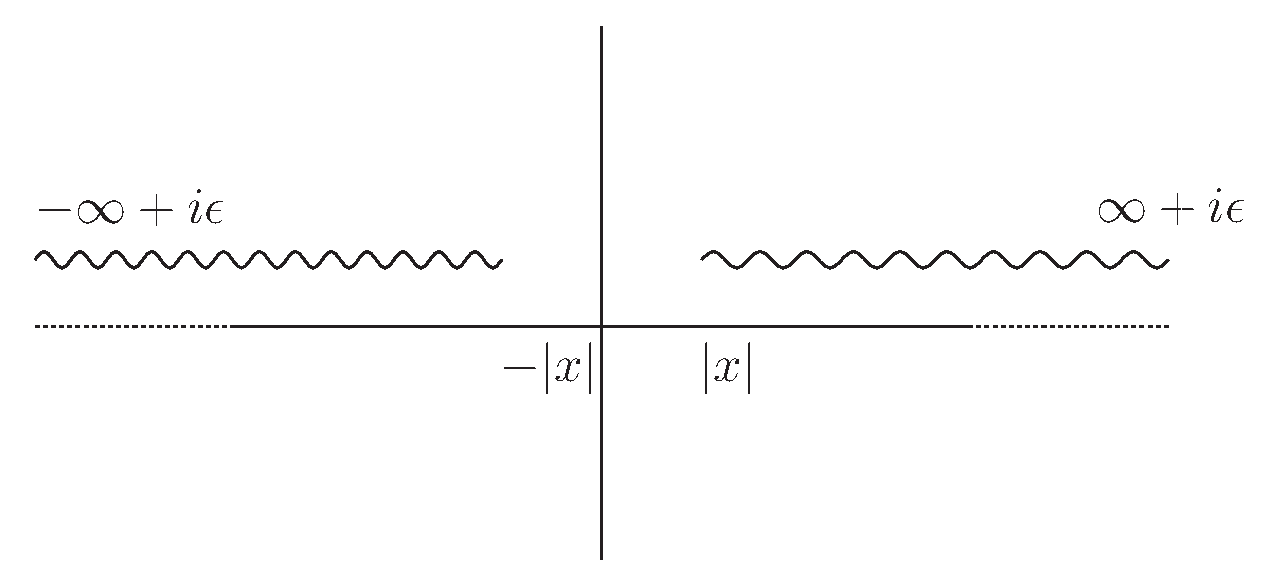
\includegraphics[width=6cm]{wightmananalyticfig.eps}
\caption{Analytic Structure}
\label{analyticwightman}
\end{subfigure}
\qquad
\qquad
\begin{subfigure}[b]{6cm}
\includegraphics[width=6cm]{wightmananalyticcontourfig.eps}
\caption{Contour of Integration}
\label{wvacontour} 
\end{subfigure}
\caption{Wightman Function}
\end{center}
\end{figure}
The analytic structure of the integrand in the $t$-plane is shown in Figure \ref{analyticwightman}. Note that there are two branch cuts, both of which lie in the upper half plane.

Let us do the $t$ integral first. Note that this integral can be taken to have a branch cut running from $(i \epsilon + \norm{x}, i \ep + \infty)$ and another one from $(i \ep - \infty, i \ep - \norm{x})$. In the case where $\omega < 0$, we can close the $t$-contour in the {\em lower half plane}, and since there are no singularities in that region, we just get $0$. Now, by the remark above, \eqref{wvacuumdef} is invariant under Lorentz transformations that are continuously connected to the identity. If $\vect{k}^2 - \omega^2 > 0$, then by using such a transformation, we can make the time component of the momentum $d$-vector negative. This immediately tells us that we need to consider \eqref{wvacuumdef} only for vectors that have
\[
\omega > 0, \quad \text{and} \quad \omega^2 - \vect{k}^2 > 0
\]

We can now transform the $t$-integral in \eqref{wvacuumdef} by deforming the original contour, which runs along the real axis to the contour shown in \ref{wvacontour}. Considering the various phases along the legs of this contour carefully, we see that this is just
\be
\label{wightmanfuncvacuumb}
G(\omega, \vect{k} ) = 2 \left( e^{i \pi \Delta} - e^{-i \pi \Delta} \right) \int d^{d-1} \vect{x} \int_{t=|\vect{x}|}^{\infty} {e^{i \omega t - i \vect{k} \cdot \vect{x}} \over |t^2 - \vect{x}^2|^{\Delta}} dt,
\ee
We now change coordinates to: $\rho^2 = t^2 - \vect{x}^2$, and write $t = \rho \cosh \zeta, |\vect{x}| = \rho \sinh \zeta$. We also choose a frame where
the vector $(\omega, \vect{k}) \rightarrow (\sqrt{\omega^2 - \vect{k}^2}, 0, 0, \ldots)$. We can then rewrite \eqref{wightmanfuncvacuumb} as
\[
\begin{split}
G(\omega, \vect{k}) &= \theta(\omega) \theta(\omega^2 - \vect{k}^2) 2 \left( e^{i \pi \Delta} - e^{-i \pi \Delta} \right) {V_{d-2}} \int {e^{i \sqrt{\omega^2 - \vect{k}^2} \rho \cosh{\zeta}} \over \rho^{2 \Delta}} \, \rho^{d-1} d\rho \, \sinh(\zeta)^{d-1} d \zeta \\ 
&\equiv N_{\Delta,d} \,\theta(\omega) \theta(\omega^2 - \vect{k}^2) (\omega^2 - \vect{k}^2) ^{\Delta - d/2}
\end{split}
 \]
where $V_{d-2}$ is the volume of the $d-2$-sphere and $N_{\Delta,d}$
is an irrelevant non-zero numerical constant that comes from the
integral over $\zeta$ and $\rho$. 

Notice that this implies that the modes ${\cal O}_{\omega,\vect{k}}$ with positive $\omega$ annihilate the vacuum, while the modes ${\cal O}_{-\omega,-\vect{k}}$ and $\omega>0$, when acting on the vacuum, create excitations of energy $\omega$ and momentum $\vect{k}$. Moreover, {\em in the vacuum}, we have for the commutator
\[
\lvac[{\cal O}_{\omega, \vect{k}}, {\cal O}_{\omega', \vect{k}'}]
\rvac = 
G(|\omega|, \vect{k})\, \text{sgn}(\omega) \,\delta(\omega+\omega') \,\delta^{d-1}(\vect{k} + \vect{k}'),
 \]
In fact, large $N$ factorization \eqref{factorization} implies that the right hand side of the equation above is unchanged if replace the vacuum  by any normalized state $|{\cal S} \rangle$  that is created by the action of only a finite number of insertions of ${\cal O}$.

At subleading orders in $N$, the spacelike modes of ${\cal O}$ are relevant, and they do not satisfy the algebra above.  This implies that if we consider the Wightman two-point function in a state with an energy that scales with $N$ (like a big black hole), then these relations stop holding as we will find below.





However, the calculation above tells us that 
{\it
\begin{quote}
At leading order in ${1 \over N}$, while computing finite-point correlators of ${\cal O}_{\omega,\vect{k}}$ about the vacuum, we can neglect the spacelike modes of ${\cal O}_{\omega,\vect{k}}.$
\end{quote}}
\noindent Moreover, if we define the operators (for $\omega > 0$ and
$\norm{k}^2 > 0$)
\[
\begin{split}
\hat{\cal O}_{\omega, \vect{k}} &= {{\cal O}_{\omega, \vect{k}} \over 
\sqrt{G(\omega,\vect{k})}},
\\
\hat{\cal O}^{\dagger}_{\omega, \vect{k}} &= {{\cal O}_{-\omega, -\vect{k}} \over 
\sqrt{G(\omega,\vect{k})}},
\end{split}
 \]
then these operators (inserted between states $|{\cal S}\rangle$ made out of finite number of insertions of ${\cal O}$) just satisfy the algebra of free oscillators
\[
[\hat{O}_{\omega, \vect{k}}, \hat{O}_{\omega', \vect{k}'}^{\dagger}] = \delta(\omega-\omega') \delta^{d-1}(\vect{k} - \vect{k}').
 \]

Physically this means that the excitations created by the action of the generalized free field ${\cal O}$ have the structure of a freely generated Fock space. However, these excitations are qualitatively different from those created by an ordinary free field. In the case of an ordinary free field $\phi$ on the boundary, the excitations are simply labeled by the $d-1$ components of their spatial momentum $\vect{k}$, while their energy is determined by $\omega = \sqrt{\vect{k}^2+m^2}$. This dispersion relation follows from the {\it equation of motion} that the ordinary free field satisfies (for example $\Box\phi = m^2\phi$). In contrast, the excitations created by a generalized free field ${\cal O}$ are labeled by $d$ independent numbers, namely $\vect{k}$ {\it and} $\omega$. Except for the condition that $\omega^2 > \vect{k}^2$, there is no constraint among them, i.e. no dispersion relation, because the generalized free field ${\cal O}$ {\it does not satisfy any wave equation on the boundary}. 
In a sense that we will make precise in the next subsection, the excitations created by a generalized free field can be reorganized as the excitations of an ordinary free field living in a higher dimensional (AdS) spacetime.

From now on, we will take $\omega$ to be positive and will always work with positive frequency modes, that is, instead of writing ${\cal O}_{-\omega,-\vect{k}}$ we will write ${\cal O}_{\omega,\vect{k}}^\dagger$.

\subsection{Local operators on the Poincare patch}
Now, consider AdS$_{d+1}$ in the Poincare patch with geometry
\be
\label{poincarepatch}
ds^2 = {-dt^2 + d\vect{x}^2 + dz^2 \over z^2}.
\ee
Notice that we are working in units where the AdS radius is set to
one. We consider a free massive scalar field propagating on this background.
The equation of motion of this field is
\be
\label{poincareeom}
(\Box -m^2)\phi=0
\ee
It is quite easy to solve \eqref{poincareeom}. The standard solution
is in terms of Bessel functions and the {\em normalizable mode} is
\be
\label{normalizablemomentum}
\xi_{\omega, \vect{k}}(t,\vect{x},z) = e^{-i\omega t + i \vect{k} \cdot
  \vect{x}} {\Gamma(1+\nu)\over \normfact}\left({2\over \sqrt{\omega^2 - \vect{k}^2} }\right)^\nu z^{d/2}J_{\nu}(\sqrt{\omega^2 - \vect{k}^2} z) ,
 \ee
where $\nu = \sqrt{m^2 + d^2/4}$.
We have chosen the overall normalization of the mode such that it behaves 
like $\normfact^{-1}\times z^\Delta \times e^{-i\omega t + i \vect{k} \cdot \vect{x}}$ near the boundary $z=0$, and we have $\Delta= \nu + d/2$. We will also take 
\be
\label{normfactdef}
\normfact = (2 \pi)^{d \over 2} \sqrt{2 {\Gamma(\Delta - {d \over 2} + 1) \pi^{d \over 2}  \over \Gamma(\Delta)}},
\ee
for later convenience.

Notice that it is possible to find normalizable modes which do not blow up at the Poincare horizon only if $\omega^2\geq \vect{k}^2$ i.e. there are no normalizable modes with spacelike momentum along the boundary directions. This is consistent with the fact that at large $N$ the spacelike Fourier modes ${\cal O}_{\omega,\vect{k}}$ can not create any excitations when acting on the vacuum, as we found above.

We can now easily write down a (nonlocal) CFT operator, which behaves like a {\em local field} in the Poincare patch. This is simply given by
\be
\label{finalpoincare}
\boxed{
\phi_{\text{CFT}}(t, \vect{x}, z) = \int_{\omega>0} {d\omega  d^{d-1} \vect{k}  \over (2 \pi)^d}\left[{\cal O}_{\omega,\vect{k}}\,\, \xi_{\omega,\vect{k}}(t,\vect{x},z) + {\cal O}^{\dagger}_{\omega,\vect{k}}\,\, \xi^*_{\omega,\vect{k}}(t,\vect{x},z) \right]}
\ee 
We use the subscript CFT to emphasize that while $\phi_{\text{CFT}}$ seems to depend on all AdS coordinates $(t,\vect{x},z)$ it is still an operator in the conformal field theory, though clearly non-local. From the point of view of the CFT, the coordinate $z$ is in a sense ``auxiliary''. It simply parameterizes how exactly we have smeared the boundary operator ${\cal O}(t,\vect{x})$ to reproduce the nonlocal operator $\phi_{\text{CFT}}(t,\vect{x},z)$. 

The main point here is that since $\phi_{\text{CFT}}$ has exactly the same expansion as that of a free massive field in AdS, it necessarily behaves --- at large $N$ --- like a local field in the ``emergent'' AdS space, which is constructed by the boundary coordinates $t,\vect{x}$ together with the parameter $z$ and equipped with the metric \eqref{poincarepatch}. For example, with the choice in \eqref{normfactdef}, we have\footnote{Our unusual choice for the normalization of this field has to do with the fact that we wanted to remove factors of $2 \pi$ from our momentum mode commutators.}
\be
[\phi_{\text{CFT}}(t, \vect{x}, z), \dot{\phi}_{\text{CFT}}(t, \vect{x'}, z')] = {i \over (2 \pi)^d} \delta^{d-1}(\vect{x} - \vect{x'}) \delta(z - z') z^{d-1}.
\ee
Moreover, the action of the conformal transformations on ${\cal O}(t,\vect{x})$ generates just an action of the isometries of AdS on $\phi_{\text{CFT}}(t,\vect{x},z)$. 


\subsection{Local operators behind the Poincare horizon}
So far what we have done is not surprising, and was already done in the works cited at the beginning of the subsection \ref{subsec:freevac}. We now show how it is possible to construct local fields on {\em global AdS} using these modes. 

Figure \ref{poincaretoglobal} shows two ways in which this may be done. 
\begin{figure}[!h]
%\label{poincaretoglobal}
\begin{center}
\begin{subfigure}[b]{6cm}
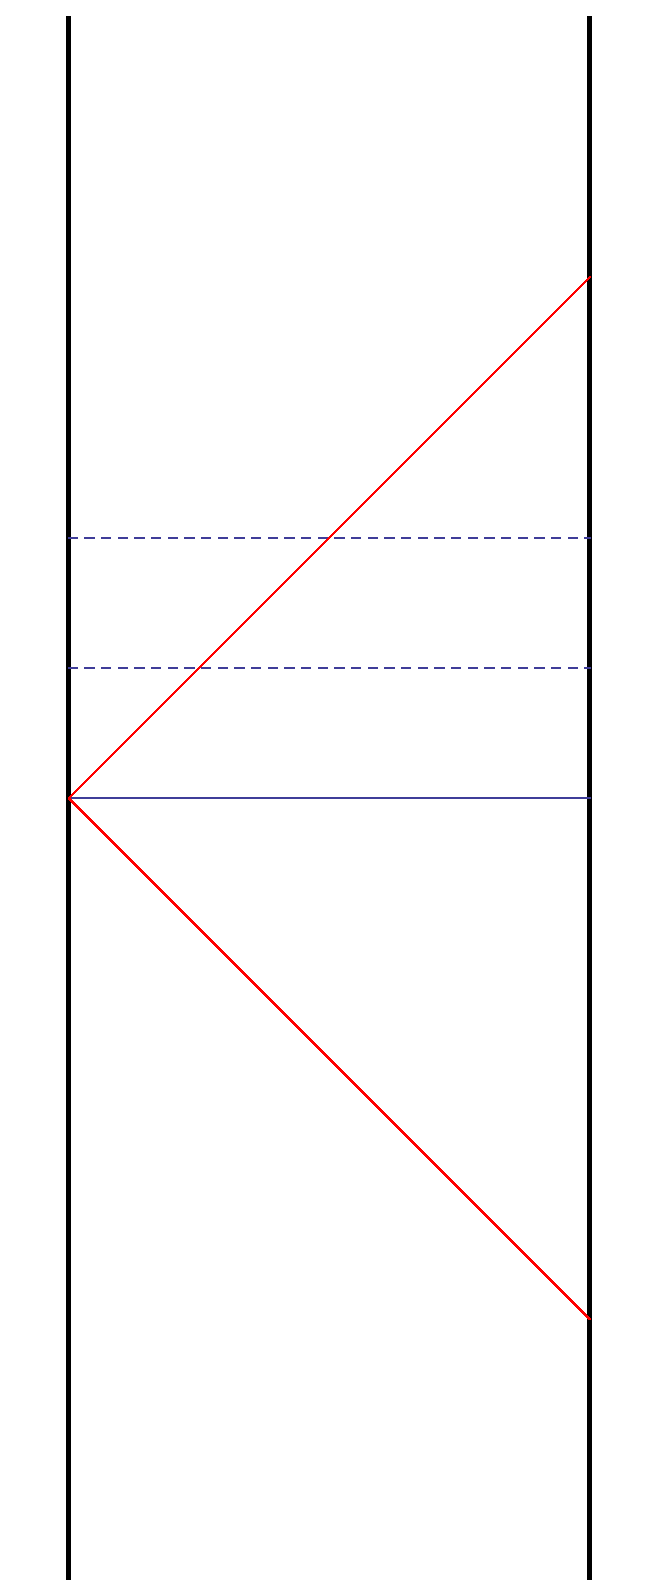
\includegraphics[width=6cm, height=5cm]{pointoglobal1}
\caption{Global time slices \label{globaltimecoord}}
\end{subfigure}
\qquad
\qquad
\begin{subfigure}[b]{6cm}
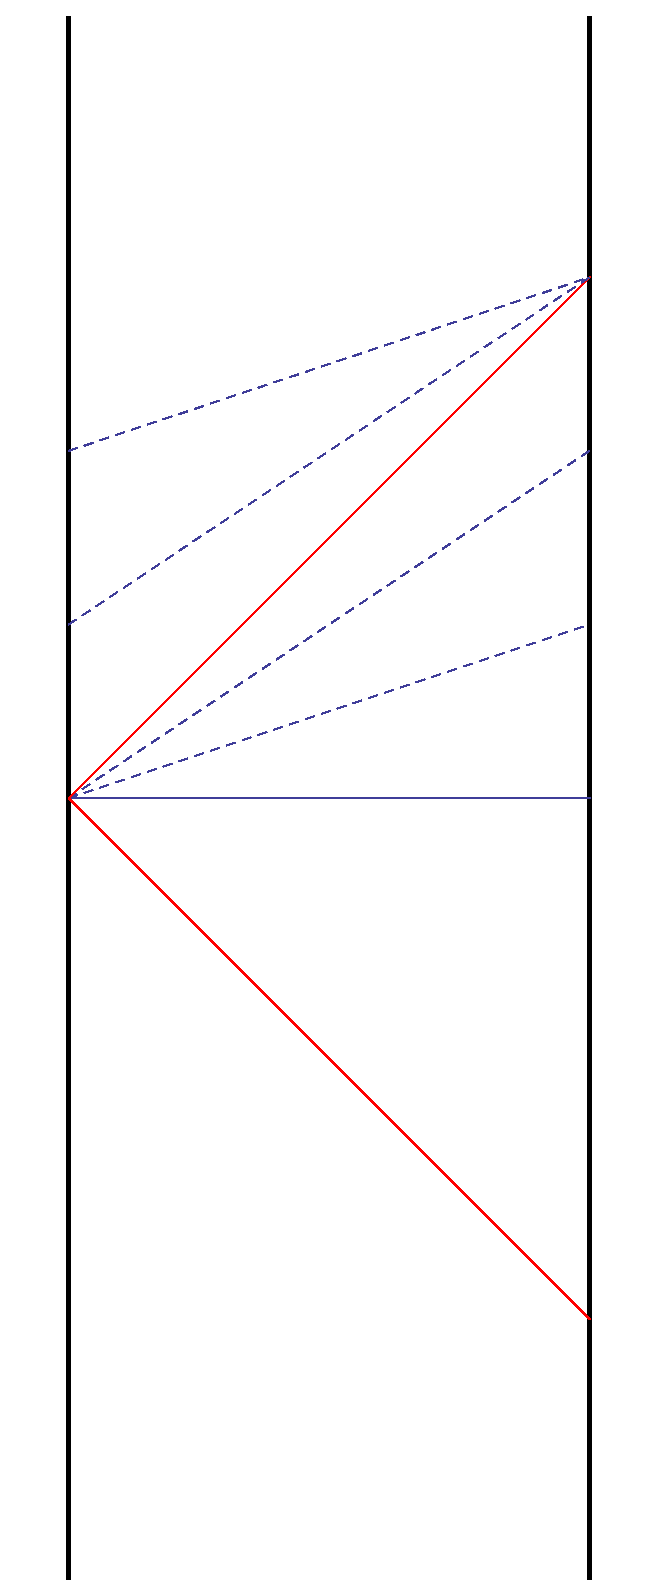
\includegraphics[width=6cm, height=5cm]{pointoglobal2}
\caption{Poincare time slices \label{pointimecoord}}
\end{subfigure}
\caption{Local operators in global AdS using the boundary of the Poincare patch \label{poincaretoglobal}}
\end{center}
\end{figure}
In the method indicated in \ref{globaltimecoord}, we first construct local operators on a Cauchy slice that lies entirely within the Poincare patch. We then use the equations of motion to evolve these operators forward in global AdS time beyond the Poincare patch. In practice, to write down an explicit local field like \eqref{finalpoincare}, we would need to do a Bogoliubov transform from the solutions to the wave equation given in \eqref{normalizablemomentum} that have a well defined energy with respect to Poincare time to solutions that have a well defined energy with respect to global AdS time. 

It is simpler to write down explicit operators using the method indicated
in figure \ref{pointimecoord}. We can quantize a field in global AdS
using the sequence of spacelike slices shown there. There is a natural
continuation of these slices beyond the future horizon. We now demonstrate this construction more precisely.

Consider global AdS written in coordinates
\[
ds^2 = -\cosh^2 \rho \,d t^2 + d \rho^2 + \sinh^2 \rho \,d \Omega_{d-1}^2
\]
The $d-1$ sphere that enters here can be parameterized in terms of $d-1$ angles and embedded in $R^d$ through $(\Omega_1, \Omega_2, \ldots \Omega_d) = (\cos \theta_1, \sin \theta_1 \cos \theta_2, \ldots \sin \theta_1 \sin \theta_2 ... \sin \theta_{d-1})$. (If $d$ is even, then the last entry has a $\cos \theta_d$ instead but this detail is not relevant below.) 

To {\em motivate our construction} of operators in this space, we write
\be
\label{globaltopoincare}
\begin{split}
t &=  \frac{\cosh \rho \sin \tau }{\cos \tau \cosh \rho + \cos \theta_1  \sinh \rho} \\
x_i &= \frac{\Omega_{i+1} \sinh\rho }{\cos \tau \cosh \rho + \cos \theta_1 \sinh\rho}, \quad i = 1 \ldots d-1 \\
z &= {1 \over \cos \tau\cosh \rho  + \cos \theta_1 \sinh \rho}
\end{split}
\ee
 The boundary, which is at $z = 0$ is clearly at $\rho = \infty$. The horizon, which is $z = \infty$ is defined by the equation
\[
\cos \tau\cosh \rho  + \sin \theta_1 \sinh \rho=0.
 \]
At the boundary, the coordinate change between $t,\vect{x}$ and $\tau, \Omega_i$ is
\[
t = {\sin \tau \over \cos \tau + \sin \theta_1}, \quad x_i = {\Omega_{i+1} \over \cos \tau  + \sin \theta_1 }.
 \]

Now we analytically continue our solutions from the Poincare patch to all of global AdS.  We take the solutions given in \eqref{normalizablemomentum} and substitute the coordinate transformation \eqref{globaltopoincare}. So, in global coordinates we write the solution
\[
\xi_{\omega,\vect{k}}(\tau, \rho, \Omega_i) = e^{-i \omega t(\tau, \rho, \Omega_i)} e^{i \vect{k} \cdot  \vect{x}(\tau, \rho, \Omega_i)}{\Gamma(1+\nu) \over \normfact}
\left({2\over \sqrt{\omega^2 - \vect{k}^2}}\right)^\nu z(\tau, \rho, \Omega_i))^{d \over 2} J_{\nu}(\sqrt{\omega^2 - \vect{k}^2} z(\tau, \rho, \Omega_i)),
\]
where the functions $t(\rho, \tau, \Omega_i), \vect{x}(\rho, \tau, \Omega_i), z(\rho, \tau, \Omega_i)$ are given by \eqref{globaltopoincare}. There is a small subtlety regarding a phase that we need to be careful about. 

When we cross $z = 0$, and go to negative $z$, we pick up a phase. This is because
\[
J_{\nu}(-x) = e^{i \pi \nu} J_{\nu}(x).
 \]
As we cross the next horizon, we should then pick up a net phase of $e^{2 \pi i \nu}$. 

With this convention, we can write down local operators in global AdS 
simply as
\be
\label{finalglobal}
\phi_{\text{CFT}}(\tau, \rho, \Omega_i) = \int_{\omega>0} {d\omega  d^{d-1} \vect{k}  \over (2 \pi)^d} \left[{\cal O}_{\omega,\vect{k}}\,\, \xi_{\omega,\vect{k}}(\tau, \rho, \Omega_i) + {\cal O}^{\dagger}_{\omega,\vect{k}}\,\, \xi^*_{\omega,\vect{k}}(\tau, \rho, \Omega_i) \right]
\ee 
The fields that we get by this construction are clearly periodic in the Poincare patch up to a phase. However, this is consistent with the fact that the equations of motion require $\phi$ to be periodic in global time, up to a phase. 

It is also easy to see that if we take the limit of this operator 
\[
\lim_{\rho \rightarrow \infty}  \left[\normfact\, e^{\rho \Delta}\,\phi_{\text{CFT}}(\tau, \rho, \Omega_i)\right] = {\cal O}^g(\tau, \Omega_i)
\]
where ${\cal O}^g$ is nothing but the continuation of the operator ${\cal O}$ from Minkowski space to its infinite sheeted covering that is conformal to  ${\mathbb S}^{d-1} \times {\mathbb R}$ and we remind the reader that 
the normalization factor $\normfact$ is given in \eqref{normfactdef}. In fact, many years ago Luscher and Mack \cite{Luscher:1974ez} showed that the correlation functions of the CFT on ${\mathbb R}^{d-1,1}$ could be continued to ${\mathbb S}^{d-1} \times {\mathbb R}$. This continuation can also be done, by first continuing to Euclidean space, and then continuing back to get the space ${\mathbb S}^{d-1} \times {\mathbb R}$. 

\paragraph{Continuing the CFT from ${\mathbb R}^{d-1,1}$ to ${\mathbb S}^{d-1} \times {\mathbb R}$}
For the benefit of the reader, we briefly review how CFTs can be
continued from Minkowski space to ${\mathbb S}^{d-1} \times {\mathbb R}$. The reader who is
already familiar with this topic can skip to the next subsection,
which has a ``discussion'' of the implications of our construction.

This extension is described very clearly in \cite{Aharony:1999ti}.  (see pp. 37--39.). We focus on the time coordinate $t$ and the spatial radial coordinate $r$ of Minkowski space. Let us compactify it down to the triangle by writing $r\pm t = \tan(\theta \pm \tau)$. This maps a triangle in the $\tau,\theta$ patch to the full $t,r$ plane. Writing $u_{\pm} = r \pm t$, we find that
\[
{\partial \over \partial \tau} = {1 \over 2} \left[(1 + u_{+}^2) {\partial \over \partial u_{+}} + (1 + u_{-}^2) {\partial \over \partial u_{-}} \right]]= {1 \over 2} \left(P_0 + K_0\right),
 \]
If we take our Hamiltonian to be ${1 \over 2}\left(P_0 + K_0 \right)$, then this Hamiltonian generates translations in $\tau$. In the $\tau, \theta$ plane we can continue correlators past  the edges of the triangle
onto the whole cylinder. 

There is another way to understand why it is this quantity that should
be used as the Hamiltonian when we go from ${\mathbb R}^{d-1,1}$ to ${\mathbb S}^{d-1} \times {\mathbb R}$. The basic point is that we can understand the action of the conformal algebra on the Hilbert space of the {\em Lorentzian theory}, by cutting up the Euclidean path integral that defines the theory in different ways. The boundary Euclidean path integral can be performed on ${\mathbb R}^d$ (or after adding a point at infinity on ${\mathbb S}^d$). We can cut this space either as ${\mathbb R}^{d-1} \times {\mathbb R}$ or as ${\mathbb S}^{d-1} \times {\mathbb R}$.\footnote{Note that both Minkowski space and the space ${\mathbb S}^{d-1} \times {\mathbb R}$ give the same space upon Euclidean continuation.} 

The Hilbert space that we get in these two ways is different, although
the theories are isomorphic. In the ${\mathbb R}^{d-1} \times {\mathbb
  R}$ slicing, states are defined by inserting an operator at
Euclidean time $-\infty$ and doing the path integral up to $0$. In the
${\mathbb S}^{d-1} \times {\mathbb R}$ slicing, states are defined by
inserting an operator at the origin and doing the path integral out to
unit radius. 

The dual of a state is defined, in the flat-space slicing, by inserting an operator at Euclidean time $+\infty$ and doing the path integral back to $0$; in the ${\mathbb S}^{d-1} \times {\mathbb R}$ slicing by inserting an operator at $\infty$ and do the path integral back to the unit sphere.

Consequently, the definition of the adjoint is different as well. In the flat-space slicing, the adjoint operation clearly leads to the hermiticity conditions
\[
P_i^\dagger = P_i; \quad P_0^{\dagger} = -P_0; \quad K_i^\dagger =
K_i; \quad K_0^{\dagger} = -K_0. 
 \]
The minus sign for the time component comes, in this language, because the mapping from bras to kets involves taking $t_{\text{euclidean}} \rightarrow -t_{\text{euclidean}}$. Here, the $i$ component runs only over spatial indices. The algebra that we get in this manner from the Euclidean path integral is isomorphic to the group $SO(d,2)$, with the usual hermiticity conditions.

On the other hand, in the ${\mathbb S}^{d-1} \times {\mathbb R}$ slicing, the mapping from bras to kets involves taking $|x| \rightarrow {1 \over |x|}$. So, the adjoint of a translation involves an inversion followed by a translation and another inversion. This leads to the Hermiticity conditions
\[
P_{\mu}^\dagger = K_{\mu}.
 \]
Hence, we get two different relations for the adjoint by changing the inner-product.







Now, instead of changing the inner product we can instead do a 
similarity transform on the operators, and keep the inner product fixed. This similarity transform is given in detail in \cite{Minwalla:1997ka}. (See section 2.1.) This gives rise to the relation that the dilatation operator in the ${\mathbb S}^{d-1} \times {\mathbb R}$ slicing is related to the operators in the ${\mathbb R}^{d-1} \times {\mathbb R}$ slicing through
\[
D^{{\mathbb S}^{d-1}} = {i \over 2} (P_0^{{\mathbb R}^{d-1}} + K_0^{{\mathbb R}^{d-1}}),
 \]
This operator is anti-hermitian, just like $P_0$ above but when we Wick rotate, we get the hermitian Hamiltonian above. 



 
\paragraph{Discussion}
Note that, from the point of a view of a CFT that lives on the boundary of Poincare AdS, this construction seems a little surprising. A common, but incorrect, belief
is that this CFT has only partial information about global AdS. To the contrary, as we have shown above, the CFT gives us {\em all bulk correlators} in global AdS. 

We have also encountered the objection that ``if someone were to turn on a source of change the Hamiltonian somewhere in global AdS beyond the Poincare patch, how would 
the flat-space CFT know about this''?  Indeed, the CFT would not be
able to account for such a ``divine intervention'' but we emphasize
that this objection could also have been raised in the original
Poincare patch. If we were to change the Hamiltonian somewhere in the bulk, this would simply change the theory away from the original CFT and without further information, we would not be able to compute these new correlators. 
  
So, our flat-space CFT describes a {\em specific} theory on the Poincare patch, and a {\em specific} theory on global AdS. It can also describe small deformations away from this theory, such as those obtained by turning on sources in the bulk since the effect of these sources can be captured by a power series expansion in the original correlators. It cannot account for arbitrary changes to the Hamiltonian but this is not unusual and holds for all examples of the AdS/CFT correspondence.
 
%%% Local Variables: 
%%% mode: latex
%%% TeX-master: "infalling_paper"
%%% End: 
